\section{Case Studies}

In this section we present a pair of example applications of the
capabilities provided by RCloud. The examples themselves are synthetic
(unfortunately, we are unable to show production notebooks because of
their business value), but the examples are representative of the
type of progression we want the ecosystem to support.

\subsection{Stock Price Analysis\label{sec:stockvis}}

\begin{figure}
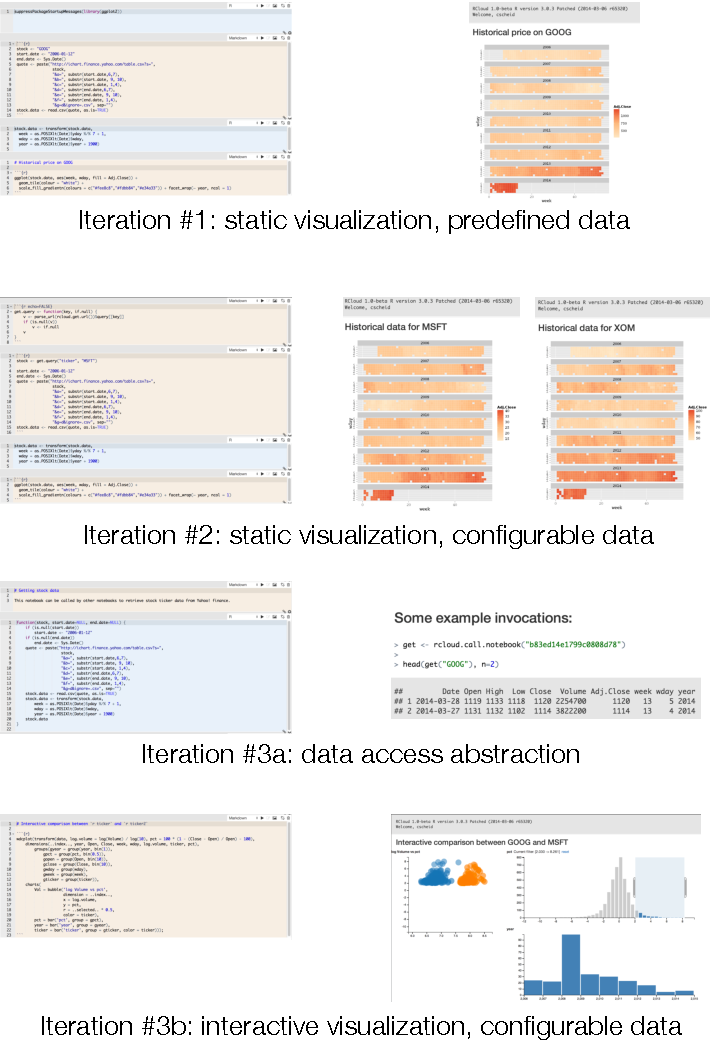
\includegraphics[width=\linewidth]{fig/casestudy1/casestudy1.pdf}
\caption{\label{sec:stockvis}Iterations of a stock ticker
  visualization, based on an example suggested by Hadley Wickham.  A
  simple, static visualization of the closing price of a single ticker
  is progressively improved into a configurable visualization suitable
  for dashboarding, then into an interactive visualization of the
  volatility and volume of two separate stocks, then finally into API
  calls for data access use in other RCloud notebooks. All notebooks
  in this can be used directly as web pages. When a notebook
  corresponding to a function call is used as a web page, its included
  documentation is displayed.}
\end{figure}

Our first example is a sequence of visualizations of the performance
of stock prices over a multi-year period. The first visualization uses
ggplot2 and is due to Hadley Wickham. It uses data provided by Yahoo!
Finance via their web service, and shows the stock price for a single
symbol.

The webpage that produces that visualization always includes a link
back to the generating source code, from which a user can always fork
the notebook and, in this case, add a configurable ticker based on the
URL of the notebook. Notice how the notebook changes very little.

From there, the notebook author (or a user) can decide to provide easy
access to the data without producing a visualization. This is achieved
by simply creating a notebook that defines a function. This notebook
then becomes a \emph{subroutine} for other notebooks, and is
version-controlled in the same way.

Interactive version.

%% This notebook can then be called in an \emph{interactive}
%% visualization, which uses the Javascript 

%% Easy to convert it into configurable entry point for dashboarding.

%% Now consider an analyst that wants to understand the price dynamics of
%% different stock attributes, different points in time, etc. For that,
%% interactive visualization is very attractive. describe dcplot and
%% notebook which uses it.

%% Then describe abstraction of stock-data fetching, to talk about
%% calling notebooks from other notebooks.

%% then call.r?

\subsection{text analysis\ref{sec:textvis}}

Same.

% IMPORTANT: what is unique about RCloud here
% From prototyping to dashboard
% Getting other information from the web
%
